\documentclass[Journal,letterpaper]{ascelike-new}
%% Please choose the appropriate document class option:
% "Journal" produces double-spaced manuscripts for ASCE journals.
% "NewProceedings" produces single-spaced manuscripts for ASCE conference proceedings.
% "Proceedings" produces older-style single-spaced manuscripts for ASCE conference proceedings. 
%
%% For more details and options, please see the notes in the ascelike-new.cls file.

% Some useful packages...
\usepackage[utf8]{inputenc}
\usepackage[T1]{fontenc}
\usepackage{lmodern}
\usepackage{graphicx}
\usepackage[figurename=Fig.,labelfont=bf,labelsep=period]{caption}
\usepackage{subcaption}
\usepackage{amsmath}
%\usepackage{amsfonts}
%\usepackage{amssymb}
%\usepackage{amsbsy}
\usepackage{newtxtext,newtxmath}
\usepackage[colorlinks=true,citecolor=red,linkcolor=black]{hyperref}
\usepackage{longtable}
\usepackage{xltabular}
\usepackage{ltablex}
%
% Please add the first author's last name here for the footer:
\NameTag{Quevedo, \today}
% Note that this is not displayed if the NoPageNumbers option is used
% in the documentclass declaration.
%
%
\newcommand{\All}{\boldsymbol A}
\newcommand{\al}{\boldsymbol a}
\newcommand{\bl}{\boldsymbol b}
\newcommand{\Bll}{\boldsymbol B}
\newcommand{\Dsdee}{\boldsymbol{D}}
\newcommand{\Dsdep}{\boldsymbol{D}^{ep}}
\newcommand{\Dsdev}{\boldsymbol{D}^{vp}}
\newcommand{\dstraine}{\boldsymbol{\dot{\varepsilon}}^{e}}
\newcommand{\dstrainp}{\boldsymbol{\dot{\varepsilon}}^{p}}
\newcommand{\dstrainv}{\boldsymbol{\dot{\varepsilon}}^{vp}}
\newcommand{\dfds}{\boldsymbol{f_\sigma}}
\newcommand{\hl}{{h_q}}
\newcommand{\Kll}{\boldsymbol K}
\newcommand{\dfdq}{{f_q}}
\newcommand{\Fl}{\boldsymbol{F}}
\newcommand{\Nll}{\boldsymbol N}
\newcommand{\Rl}{\boldsymbol{R}}
\newcommand{\straine}{\boldsymbol{\varepsilon}^{e}}
\newcommand{\strainp}{\boldsymbol{\varepsilon}^{p}}
\newcommand{\strainvp}{\boldsymbol{\varepsilon}^{vp}}
\newcommand{\strainpeq}{\bar \varepsilon^p}
\newcommand{\strainvpeq}{\bar \varepsilon^{vp}}
\newcommand{\zerol}{\boldsymbol 0}

\newcommand{\dPhidsl}{\boldsymbol{\Phi_{_\sigma}}}
\newcommand{\dPhidql}{\boldsymbol{\Phi_{_q}}}


\newcommand{\sll}{\boldsymbol{s}}
\newcommand{\ul}{\boldsymbol u}
\newcommand{\onell}{\boldsymbol{1}}
\newcommand{\dgds}{\boldsymbol{g_\sigma}}
\newcommand{\gllum}{\boldsymbol {g_{_1}}}
\newcommand{\glldois}{\boldsymbol {g_{_2}}}
\newcommand{\glltres}{\boldsymbol {g_{_3}}}

%
%
% Mathematical Symbols
\newcommand{\deviator}{\boldsymbol{s}}
\newcommand{\Disoliel}{\boldsymbol{D}}
\newcommand{\Disolielmod}{\boldsymbol{D^{*}}}
\newcommand{\dstrain}{\boldsymbol{\dot{\varepsilon}}}
\newcommand{\dstraincr}{\boldsymbol{\dot{\varepsilon}}^{cr}}


\newcommand{\dstraineq}{\dot{\bar{\varepsilon}}}
\newcommand{\dstrainsh}{\boldsymbol{\dot{\varepsilon}}^{sh}}
\newcommand{\dstrainvp}{\boldsymbol{\dot{\varepsilon}}^{vp}}
\newcommand{\dstress}{\boldsymbol{\dot{\sigma}}}
\newcommand{\flowtensorf}{\frac{\partial\fvp}{\partial\stress}}
\newcommand{\flowtensorg}{\frac{\partial\gvp}{\partial\stress}}
\newcommand{\fo}{f_0}
\newcommand{\fvp}{f^{vp}}
\newcommand{\gvp}{g^{vp}}
\newcommand{\Jtwo}{J_{2}}
\newcommand{\onefour}{\boldsymbol{I}}
\newcommand{\qvp}{\boldsymbol{q}^{vp}}
\newcommand{\sphericaltensor}{\boldsymbol{1}\otimes\boldsymbol{1}}
\newcommand{\strain}{\boldsymbol{\varepsilon}}
\newcommand{\straincr}{\boldsymbol{\varepsilon}^{cr}}

\newcommand{\strainsh}{\boldsymbol{\varepsilon}^{sh}}
\newcommand{\strainshCEB}{\varepsilon_{sh}}
\newcommand{\stress}{\boldsymbol{\sigma}}
\newcommand{\stresseq}{\bar{\sigma}}
\newcommand{\stressy}{\sigma_{y}}
\newcommand{\unitarytensor}{\boldsymbol{1}}
\newcommand{\young}{E}
%
\begin{document}

% You will need to make the title all-caps
\title{Finite element implementation of an elastoplastic-viscoplastic constitutive law for tunnels}

\author[1]{Felipe Pinto da Motta Quevedo}
\author[2]{Denise Bernaud}
\author[3]{Samir Maghous}

\affil[1]{M.S.,Federal University of Rio Grande do Sul/PPGEC, av. Osvaldo Aranha, 99, Zip-Code 90.035-190, Porto Alegre/RS Brazil. Email: motta.quevedo@ufrgs.br}
\affil[2]{Ph.D.,Federal University of Rio Grande do Sul/PPGEC, av. Osvaldo Aranha, 99, Zip-Code 90.035-190, Porto Alegre/RS Brazil. Email: denise.bernaud@ufrgs.br}
\affil[3]{Ph.D.,Federal University of Rio Grande do Sul/PPGEC, av. Osvaldo Aranha, 99, Zip-Code 90.035-190, Porto Alegre/RS Brazil. Email: samir.maghous@ufrgs.br}

\maketitle

% Please include an abstract:
\begin{abstract}
The paper presents an efficient numerical integration scheme for coupled elastoplasticity-viscoplastiticy constitutive behavior with internal-state variables standing for irreversible processes. In most quasi-static structural analyses, the solution to boundary value problems involving materials that exhibit time-dependent constitutive behavior proceeds from the equations integration handled at two distinct levels. On the one hand, the first or local level refers to the numerical integration at each Gaussian point of the rate constitutive stress/strain relationships. For a given strain increment, the procedure of local integration is iterated for stresses and associated internal variables until convergence of the algorithm. On the other hand, the second or global level is related to structure equilibrium between internal and external forces achieved by the Newton-Raphson iterative scheme. A review of the elastoplastic and viscoplastic model will be shown, following the coupling between these models. Particular emphasis is given in this contribution to address the first level integration procedure, also referred to as algorithm for stress and internal variable update, considering a general elastoplastic-viscoplastic constitutive behavior. The formulation is described for semi-implicit Euler schemes. The efficacy of the numerical formulation is assessed by comparison with analytical solution derived for deep tunnel in coupled elastoplasticity-viscoplascitity.
\end{abstract}

\section{Introduction}
Deep tunnels are those whose deformation field, induced by excavation, does not significantly reaches the surface. The field of strain and stresses around the cavity of deep tunnel depends on several interrelated factors, such as the depth of the tunnel, the geometry of the cross section, the anisotropy of stresses in situ, the heterogeneity of the rock mass, the coupling between the rock mass and the lining during the construction of the tunnel and the mechanical behavior of the rock mass and lining. In general, for both the rock mass and the lining, several developments in literature of the rheological models are found whose parameters are adjusted based on samples tests.

An elastoplastic-viscoplastic constitutive law becomes important when the material behavior can’t be describe by the usual models like elastoplasticity or viscoplastic. This problem is characteristic of deep tunnels excavated in clay rockmass as described by \citeN{Rousset1988}. In these cases plastification around the rockmass, gradual closing of the tunnel section, extrusion of the excavation face and overloading on the lining can develop over the construction time (short term), or even months and years after the construction of the tunnel (long term), which can lead to excessive deformations \cite{barla2008}, entrapment of the machine \cite{ramoni2010} and damage to the lining.
In addition to the present work, elastoplastic-viscoplastic models applied to the problem of deep tunnels can be found in: \citeN{Rousset1988}, \citeN{piepi1995}, \citeN{Purwodihardjo2003}, \citeN{kleine2007}, \citeN{shafiqu2008}, \citeN{debernardi2009}, \citeN{souley2011}, \citeN{mahn2015}.
This work presents a numerical integration scheme for the elastoplastic-viscoplastic constitutive behavior.
For that, a brief bibliographical review will be made about each model separately and later its coupling.
Finally, the validation of this model will be presented, comparing its numerical solution with the analytical and numerical solution obtained by \citeN{piepi1995} of an excavated tunnel under axisymmetric conditions.









%For the rockmass, \citeN{boidy2002back} applied the \citeN{Lemaitre:1996} model, using a finite difference model in axisymmetry, at the Mont Terri reconnaissance gallery. \citeN{shalabi2005fe}, compares potential and hyperbolic creep models in the Stillwater tunnel with axisymmetric models. They came to the conclusion that the power law model provides better results if the lining placement delay time is considered. \citeN{sterpi2009visco}, through a parametric study, investigate a viscoelastic-viscoplastic rheological model with damage parameter, to capture the three creep stages. \citeN{pellet20093d}, with an explicit 3D numerical model, investigates the damage zone of the excavation, considering Lemaitre's viscoplastic model \citeyear{Lemaitre:1996} with a damage parameter. They shows limitations of this model and affirm that the time-dependent behavior of concrete needs to be taken into account. \citeN{barla2012time} analyzes two viscoelastic-viscoplastic laws in the Saint Martin La Porte access to the Lyon-Torino Base Tunnel under axisymmetric conditions. They concluded the need for an accurate description of the construction process.

%For the lining, \citeN{lackner2002hybrid} investigate the influence of lining stress controllers on shotcrete lining. \citeN{Collota:2010}, through experimental measurements in a pilot tunnel, studied the behavior of shotcrete, with different dosages and accelerators, coupled with steel ribs. \citeN{arnau2012longitudinal}, using creep coefficients, analyze residual longitudinal internal force in the lining after its long-term deformations. \citeN{schadlich2014application} present the application of an elastoplastic model for shotcrete, whose modulus of elasticity and strength are given by CEB-FIP MC90 as a function of time. \citeN{neuner2018formulation} compare their model whose creep was based on a modification of the Solidification Theory of \citeN{bazant:1989a} with two other models, \citeN{meschke1996numerical} and \citeN{schadlich2014application}.

%Despite these developments, there are no studies about the interaction of the rheological behavior of the lining with viscous rock mass. Thus, the aim of this study is to investigate the influence of some of the main parameters of deep concrete-lined tunnels in long-term convergence.

%In a phenomenological way, the creep in the concrete represents a dimensional change in the material under the influence of the sustained loading while the shrinkage is the decrease in volume caused by drying. Creep and shrinkage are complex phenomena and have a considerable impact on the performance of the concrete lining and in the long-term convergence of tunnel, causing strain and stress distribution around the cavity of tunnel.

%The viscoelastic lining is implemented in ANSYS using the USERMAT customization feature \cite{ANSYS:2013b}. The shrinkage is given by the CEB-FIP MC90 formulation in \cite{CEB:1993}, and the creep is modelled through a Solidification Theory of Bažant and Prassannan \citeyear{bazant:1989a,bazant:1989b} adapted to CEB-FIP MC90 formulation. This approach, which uses a Generalized Kelvin chain, is numerically convenient for modelling creep as it avoids keeping the stress history during analysis. In addition, instead of using tests to calibrate the viscoelastic model, it is proposed to use CEB-FIP MC90 formulation, which is more convenient for parametric studies.  

%The Perzyna’s viscoplastic constitutive model with an associated flow rule with von-Mises yield surface is considered for rock mass. This model was chosen because it was the only one implemented in ANSYS. There are viscoplastic models more convenient for rock mass, which uses, for example, Mohr-Coulomb \textcolor{red}{or Hoek-Brown} yield surface and non-associated flow rules.

%A total of 256 calculations have been performed using the finite element method with axisymmetric hypothesis. The excavation process is simulated by the deactivation and activation method which allow to consider the viscoplastic deformations in the surrounding rock mass before the lining installation. 

\section{Elastoplastic constitutive model}

For problems with isothermal evolution, quasi-static in small transformations, the elastoplastic constitutive model can be described through the decomposition of the total strain tensor, the flow surface, the plastic flow rule, the hardening-softening law and the conditions of loading-unloading.

\subsection{Decomposition of the total strain tensor}

Considering the hypothesis of small transformations (which includes the hypothesis of small strains) we have that the total strain rate can be decomposed into an elastic and a plastic component:
\begin{equation} \label{eq_decomposition_plastic}
    \dstrain=\dstraine + \dstrainp\;.
\end{equation}

Within the context of deterministic thermodynamic processes, the specific free energy, considering an isothermal evolution, can be decomposed according to:
\begin{equation} \label{eq_specific_free_energy}
    \psi(\strain,\strainp,\alpha) = \psi^e(\strain-\strainp)+\psi^p(\alpha) = \psi^e(\strain^e)+\psi^p(\alpha)\;,
\end{equation}
where $\alpha$ is the set of internal variables (cohesion, friction angle…) related to the hardening-softening phenomenon. From Eq.~(\ref{eq_specific_free_energy}), the following constitutive relationships are obtained:

\begin{equation} \label{eq_constitutive_relationship_plastic_free_energy}
    \stress = \dfrac{\partial \psi^e}{\partial \straine}, ~~~ q = \dfrac{\partial \psi^p}{\partial \alpha}\;,
\end{equation}
where $q$ is the set of thermodynamic forces associated with internal variables (scalar or tensor). From Eq.~(\ref{eq_decomposition_plastic}) and Eq.~(\ref{eq_constitutive_relationship_plastic_free_energy}) the following constitutive relationship is obtained:

\begin{equation} \label{eq_constitutive_relationship_plastic}
    \dstress = \Dsdep : \dstrain = \Dsdee : \dstraine = \Dsdee : (\dstraine - \dstrainp)\;,
\end{equation}
where $\Dsdee$  and $\Dsdep$ are fourth-order tensors representing the elastic and elastoplastic modulus, respectively.

\subsection{Flow surface}

A phenomenological characteristic observed in elastoplastic
materials is the existence of a limit within which the material behaves elastically. In isotropic materials, this domain is delimited by a hypersurface in the space of principal stresses, as follows:
\begin{equation} \label{eq_hypersurface}
    \partial \Gamma = \left\{ \stress | f(\stress,q) = 0 \right\}\;,
\end{equation}
where $f$ is the flow function. This surface delimits the set of stresses that are elastically admissible (E.A.) and the set of stresses that are plastically admissible (P.A.) as follows:
\begin{equation} \label{eq_PA_domain}
    \Gamma = \left\{ \stress | f(\stress,q) < 0 \right\}~\text{(E.A)}, ~ \Gamma = \left\{ \stress | f(\stress,q) \leq 0 \right\}~\text{(P.A)}\;.
\end{equation}

Fig.~\ref{fig-PA-domain} illustrates, in a generically way, this domain.
\begin{figure}
\centering
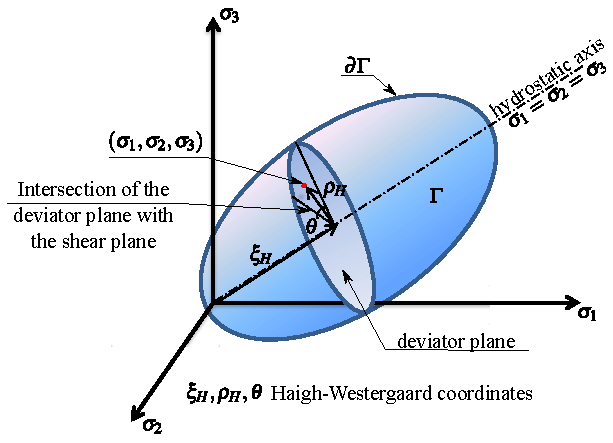
\includegraphics[scale=1]{PA-domain.pdf}
\caption{Domain plasticly admissible $\Gamma$ in the principal stress space.}
\label{fig-PA-domain}
\end{figure}

The flow function is commonly described as a function of the invariants of the stress tensor and the forces associated with the internal variables related to the hardening and softening phenomenon, so that
\begin{equation} \label{eq_flow_function_representation}
	f(\stress,q) = f(I_1,J_2,J_3,q) = f(\xi_{H},\rho_{H},\theta,q) = f(p,q^{eq},\theta,q) = f(\stress_{oct},\tau_{oct},\theta,q)\;,
\end{equation}
with
\begin{equation} \label{eq_invariants_elements}
	\begin{array}{lcl}
		I_1 = \text{tr}(\stress) = \sigma_{11}+\sigma_{22}+\sigma_{33}\\
		J_2 = \dfrac{1}{2}\text{tr}(\sll^2) = \dfrac{1}{6}\left[ (\sigma_{11}-\sigma_{22})^2 + (\sigma_{22}-\sigma_{33})^2 + (\sigma_{33}-\sigma_{11})^2 \right] + \sigma_{12}^2+ \sigma_{23}^2+ \sigma_{13}^2, \\
		J_3 = \dfrac{1}{3}\text{tr}(\sll^3) = \text{det}(\sll) = s_{11}s_{22}s_{33}-s_{11}\sigma_{23}^2-s_{22}\sigma_{13}^2-s_{33}\sigma_{12}^2+2\sigma_{12}\sigma_{23}\sigma_{13}, \\ 
		\xi_{H} = p = \sigma_{oct} = \dfrac{1}{3}I_1, ~~~ \rho_{H} = \sqrt{\sll:\sll} = \sqrt{2J_2}, ~~~ \theta = \dfrac{1}{3}\text{asin}\left( \dfrac{-3\sqrt{3}}{2} \dfrac{J_3}{J_2^{3/2}} \right), \\
		-\dfrac{\pi}{6} \le \theta \le \dfrac{\pi}{6}, ~~~q^{eq} = \sqrt{\dfrac{3}{2}\sll:\sll} = \sqrt{3J_2}, ~~~\tau_{oct} = \sqrt{\dfrac{3}{2}J_2},~~~\text{and}~~~\sll = \stress - \dfrac{p}{3}\onell.
	\end{array}\;
\end{equation}

In Eq.~(\ref{eq_flow_function_representation}), $I_1$ is the first invariant of the stress tensor, $J_2,J_3$ is the second and the third invariant of the deviator tensor $\sll$, $(\xi_{H},\rho_{H},\theta)$ are the coordinates of Haigh-Westergaard
(where $\theta$ is also known as the angle of Lode), $p$ is the hydrostatic pressure, $q^{eq}$ is the equivalent stress of von-Mises,  $(\stress_{oct},\tau_{oct})$ the normal stress and the octahedral shear, respectively \cite{chen1988}.

When the flow function does not depend of $I_1$, it is said that the plasticity is independent of pressure, being determined only by the state of stresses along the desviator plane (Fig.~\ref{fig-PA-domain}). Several flow functions can be found in the literature as in \citeN{chen1988}, \citeN{souzaneto2008} and \citeN{zienkiewicz1974}. Here is used the Drucker-Prager flow surface as:

\begin{equation}
	\label{eq:f_Drucker_Prager}
	f(\stress,q) = f(I_1,J_2,\beta_i) = \beta_1 I_1 +\beta_2 \sqrt{J_2}-\beta_3,
\end{equation}
where the $\beta_i$ parameters are related to the $c$ cohesion and the $\phi$ friction angle of the Mohr-Coulomb model. For the case where the surface of Drucker-Prager coincides with the surface of Mohr-Coulomb by the outer edges (DP-I) \cite{bernaud1991}:
\begin{equation}
	\label{eq:f_DP_circunscrita_MC}
	\beta_1 = \dfrac{(k-1)}{3}, ~~~ \beta_2 = \dfrac{(k+2)}{\sqrt{3}}, ~~~
	\beta_3 = 2\sqrt{k}~c,
\end{equation}
where $k = (1+sin{\phi})/(1-sin{\phi})$. For the case where the surface of Drucker-Prager is inscribed on the surface of Mohr-Coulomb (DP-II) \cite{bernaud1991}:
\begin{equation}
	\label{eq:f_DP_inscrita_MC}
	\beta_1 = \dfrac{(k-1)}{3}, ~~~ \beta_2 = \dfrac{(2k+1)}{\sqrt{3}}, ~~~
	\beta_3 = 2\sqrt{k}~c,
\end{equation}

\subsection{Plastic flow rule}

The law of evolution of plastic deformation (known as plastic flow rule) is postulated as
\begin{equation} \label{eq_plastic_flow}
	\strainp = \dot \lambda \gvp ~~~ \text{with} ~~~ \dgds = \dfrac{\partial g}{\partial \stress} \;,
\end{equation}
where $\lambda$ is the plastic multiplier and $\dgds$ is the tensor that gives the direction of plastic flow through the gradient of a potential function $g$ analogous to $f$. Like the flow function, the plastic potential is usually described using the invariants of the stress tensor and $\dgds$ can be determined using the chain rule. For example, if $g(I_1,\sqrt{J_2},J3,q)$ as in \citeN{viladkar1995}, we have:
\begin{equation} \label{eq_direction_plastic_flow}
	\begin{array}{lcl}
	\dgds = C_1\gllum + C_2\glldois + C_3\glltres, \\ 
	\gllum = \dfrac{\partial I_1}{\partial \stress} = \onell,~~~ \glldois = \dfrac{\partial \sqrt{J_2}}{\partial \stress} = \dfrac{1}{2\sqrt{J_2}}\sll,~~~ \glltres = \dfrac{\partial J_3}{\partial \stress}, \\
	C_1 = \dfrac{\partial g}{\partial I_1},~~~C_2=\dfrac{\partial g}{\partial \sqrt{J_2}}-\dfrac{\tan{(3\theta)}}{\sqrt{J_2}}\dfrac{\partial g}{\partial \theta},~~~C_3 = -\dfrac{\sqrt{3}}{2\cos{(3\theta})}\dfrac{1}{J_2^{3/2}}\dfrac{\partial g}{\partial \theta} \,
\end{array}
\end{equation}

As can be seen in Eq.~(\ref{eq_direction_plastic_flow}), the constants $C_1, C_2$ and $C_3$ are particularities of each type of potential function. In \citeN{viladkar1995} it is possible to obtain the value of these constants for several functions, such von-Mises, Tresca, Drucker-Prager, Mohr-Coulomb, Cap Models, etc. For Drucker-Prager potential flow has $C_1 = \beta_1$, $C_2 = \beta_2$, $C_3 = 0$.

A common aspect in geomechanics is the variation of the volume of the material during the evolution of plastic deformations. This effect is commonly introduced through unassociated plasticity, adopting, instead of the friction angle a angle of dilatance $0<\psi<\phi$ in the potencial function $g$.

\subsection{Hardening-Softening law}

The hardening-softening law characterizes the dependence of internal variables during the evolution of plastic deformations. This law is postulated as follows:

\begin{equation} \label{eq_hardening_law}
	\dot q = \dot \lambda \hl(\stress,q) = - \dot \lambda \dfrac{\partial h}{\partial q}\;,
\end{equation}
where $\hl = -\partial h / \partial q$ is a gradient of a potential fucntion $h$ with respect to the associated thermodynamic forces $q$. As the flow function $f$ is dependent on $q$, changing along the plastic deformation will change the position and/or shape of the flow surface. When the flow surface is static, that is, $\dot q = 0$, there is perfect plasticity, when increases, there is isotropic hardening and when it moves, there is kinematic hardening, being mixed, when composed of the last two. The associated hardening/softening law ($h=f$) and isotropic is considered. The associated thermodynamic force is given exclusively by the portion that does not depend on the hydrostatic ($I_1$) or deviating ($J_2$) part on the flow surfaces. This force is controlled by the cohesive parameter, so $q = \chi c(\strainpeq) = 2\sqrt{k}c(\strainpeq)$, where $\strainpeq$ is the state variable. For cohesion, it is considered a linear function defined by parts, as Eq.~(\ref{eq_cohesive_law}), in order to represent the characteristic hadrening/softening of the rock mass.

\begin{equation} \label{eq_cohesive_law}
c (\bar \epsilon^p) = \left\{ 
\begin{array}{ll} 
	c_i + \dfrac{(c_p-c_i)}{\bar \epsilon^p_I}\bar \epsilon^p &  \text{for zone I} \\ 
	c_p, & \text{for zone II} \\
	c_p + \dfrac{(c_r-c_p)}{\bar \epsilon^p_r-\bar \epsilon^p_{II}}(\bar \epsilon^p - \bar \epsilon^p_{II}), & \text{for zone III} \\	
	c_r, & \text{for zone IV}
\end{array}\right..
\end{equation}

Therefore, using the chain rule in Eq.~(\ref{eq_hardening_law}) we have 
\begin{equation}
	\label{eq:expressao_amolecimento}
	\dot q = - \dot \lambda \dfrac{\partial h}{\partial q} = - \dot \lambda \dfrac{\partial f}{\partial q} = \dot \lambda \left(- \dfrac{\partial f}{\partial q}\dfrac{\partial q}{\partial c}\dfrac{\partial c}{\partial \bar \epsilon^p}\right) = \dot \lambda \left(\chi \dfrac{\partial c}{\partial \bar \epsilon^p}\right),	
\end{equation}
where
\begin{equation}
	\label{eq:dqde}
	\dfrac{\partial c}{\partial \bar \epsilon_{p}} = \left\{ \begin{array}{ll} \dfrac{(c_p-c_i)}{\bar \epsilon^p_I} &  \text{for zone I} \\ 
		0, & \text{for zone II} \\
		\dfrac{(c_r-c_p)}{\bar \epsilon^p_{r}-\bar \epsilon^p_{II}}, & \text{for zone III} \\	
		0, & \text{for zone IV}
	\end{array}\right..
\end{equation}

The equivalent plastic deformation is calculated from the following expression:
\begin{equation}
	\label{eq:epsPeq}
	\dot{{\bar \epsilon}}^p = C||\dot \strainp||,
\end{equation}
where
\begin{equation}
	\label{eq:epsPeq}
	||\dot \strainp|| = \sqrt{(\dot{\varepsilon}^{p}_{11})^2 + (\dot{\varepsilon}^{p}_{22})^2 + (\dot{\varepsilon}^{p}_{33})^2 + 2(\dot{\varepsilon}^{p}_{12})^2 + 2(\dot{\varepsilon}^{p}_{23})^2 + 2(\dot{\varepsilon}^{p}_{13})^2}
\end{equation}
and 
\begin{equation}
	\label{eq:Czao}
	C = \dfrac{\beta_1+1/\sqrt{3}}{\sqrt{3\beta_1^2+1/2}}.
\end{equation}

When $\phi = 0$ the rockmass is independent of the hydrostatic pressure $\beta = 0$ and $C = \sqrt{2/3}$.

\subsection{Loading and unloading conditions}

The evolution of Eq.~(\ref{eq_plastic_flow}) and Eq.~(\ref{eq_hardening_law}) are subject to three conditions (conditions of Kuhn-Tucker), which are:
\begin{equation}
	\label{eq:kuhntucker}
	f \le 0,~~~ \dot \lambda \ge 0, ~~~ \dot \lambda f = 0.
\end{equation}

These conditions establish that plastic flow only occurs when the state of stresses is on the flow surface and, in this case, there is no variation of the flow function in relation to the stresses, that is:
\begin{equation}
	\label{eq:consistencia}
	\dot f = \dfrac{\partial f}{\partial \stress}:\dot \stress + \dfrac{\partial f}{\partial q}\cdot \dot q = \dfds:\dot \sigma + \dfdq \cdot \dot q = 0.
\end{equation}

Eq.~(\ref{eq:consistencia}) is known as the consistency condition.

\subsection{Plastic multiplier and continuous Elastoplastic Module}

Introducing Eq.~(\ref{eq:consistencia}) to Eq.~(\ref{eq_constitutive_relationship_plastic}) and Eq.~(\ref{eq_hardening_law}), together with Eq.~(\ref{eq_plastic_flow}), and isolating the plastic multiplier, we have:
\begin{equation}
	\label{eq:lambda}
	\dot \lambda = \dfrac{\dfds:\Dsdee:\dot \strain}{\dfds:\Dsdee:\dgds-\dfdq \cdot \hl}
\end{equation}
that introducing in the constitutive relation Eq.~(\ref{eq_constitutive_relationship_plastic}) leads to
\begin{equation}
	\label{eq:Dep}
	\Dsdep = \Dsdee - \dfrac{\left(\Dsdee:\dgds \right)\otimes\left(\dfds:\Dsdee \right)}{\dfds:\Dsdee:\dgds-\dfdq \cdot \hl}
\end{equation}
where $\otimes$ is the tensorial product.

\section{Viscoplastic constitutive model}

\subsection{Decomposition of the strain tensor}

The viscoplastic constitutive model has a rationale similar to that of elastoplasticity, which leads to the following relationship:
\begin{equation} \label{eq_constitutive_relationship_plastic}
	\dstress = \Dsdev : \dstrain = \Dsdee : \dstraine = \Dsdee : (\dstraine - \dstrainv)\;
\end{equation}
where $\Dsdev$ is the viscoplastic fourth order tensor.

\subsection{Flow surface}

Viscoplasticity does not always have an elastic domain, for example, at high temperatures certain materials can always flow under stress, that is, the flow function is zero. For these materials there are explicit functions. However, in problems involving deep tunnels, the phenomenon occurs from a certain level of stress, as described by \citeN{Rousset1988}. For these cases, surfaces $f^{vp}$ similar to those of elastoplasticity are used.

\subsection{Viscoplastic flow rule and hadrening-softening law}

Analogous to elastoplasticity, the viscoplastic flow rule and the hardening-softening law are postulated as follows:

\begin{equation} \label{eq_plastic_flow_rule}
	\begin{array}{lcl}
		\strainvp = \dot \lambda^{vp} \dgds^{vp} ~~~ \text{with} ~~~ \dgds = \dfrac{\partial g^{vp}}{\partial \stress}, \\ 
		\dot q^{vp} = \dot \lambda^{vp} \hl(\stress,q^{vp}) = - \dot \lambda^{vp} \dfrac{\partial h^{vp}}{\partial q^{vp}} ~~~\text{and} ~~~ \strainvpeq = \int_{0}^{t} \dot \lambda^{vp} dt  \,.
	\end{array}
\end{equation}

However, in this work , the viscoplasticity is perfect, that is, $\dot q^{vp} = 0$.

\subsection{Viscoplastic multiplier}

Unlike elastoplasticity, viscoplastic deformation occur even when $f^{vp} > 0$, and therefore, the consistency condition is not imposed. Thus, the rate of the viscoplastic multiplier $\lambda^{vp}$ cannot be obtained from a condition like $\dot f^{vp} = 0$ . Therefore, there are models that provide an explicit expression for  and in this work Perzyna model \cite{perzyna1966} will be adopted, as described in \citeN{zienkiewicz1974}:

\begin{equation} \label{eq_perzyna_model}
	\dot \lambda^{vp} = \dfrac{\Phi(\stress,q^{vp})}{\eta}~~~\text{and}~~~\Phi = \left\langle  \dfrac{f(\stress,q^{vp})}{f_0} \right\rangle^n \,
\end{equation} where $\Phi$ is the overstress function, $\eta$ is the dynamic viscosity constant, $n$ is the dimensionless parameter that gives the form of the power law , $f_0$ a parameter conveniently adopted and $\left\langle * \right\rangle$ is the McCauley function which is null when $* <0$ , that is, viscoplastic flow will only occur when the criterion is positive.

\section{Elastoplastic-Viscoplastic constitutive model}

The proposed elastoplastic-viscoplastic model is constructed by the serial association of the constitutive models described above, and, therefore, we have:
\begin{equation} \label{eq_constitutive_relationship_plastic}
	\dstress = \Dsdev : \dstrain = \Dsdee : \dstraine = \Dsdee : (\dstraine - \dstrainv)\;.
\end{equation}

This association can be seen in the one-dimensional representation of Fig.~\ref{reological_scheme}. An important observation is that the flow surfaces and the internal variables that define the elastoplastic and viscoplastic portion of this model can be different from each other, including the association of their respective potential functions with their flow surfaces. Generally, viscoplasticity parameters are chosen so that its viscoplastic surface is inside the elastoplastic-viscoplastic surface, thus having the domains represented in Fig.~\ref{surfaces_epvp}.

\begin{figure}
	\centering
	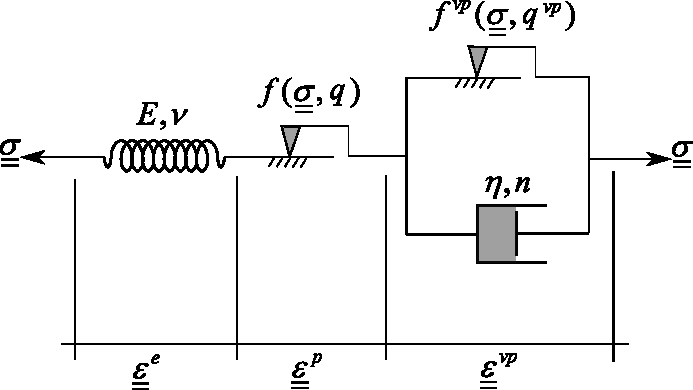
\includegraphics[scale=1]{reological_scheme.pdf}
	\caption{Rheological representation of the elastoplastic-viscoplastic model.}
	\label{reological_scheme}
\end{figure}
\begin{figure}
	\centering
	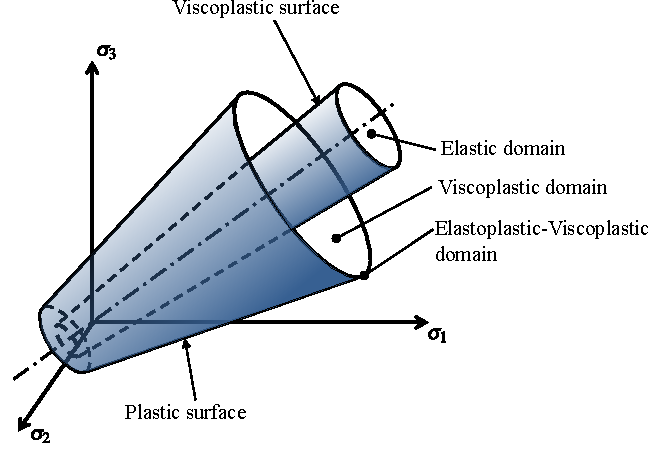
\includegraphics[scale=1]{surfaces_epvp.pdf}
	\caption{Domains and surfaces of the elastoplastic-viscoplastic model.}
	\label{surfaces_epvp}
\end{figure}

\section{Solution of nonlinear constitutive problems in finite elements}

Though the weak form of the field equations that govern the problem and the spatial discretization of the domain in finite elements, for quasi-static problems, isothermal in small transformations, we have the following set of nodal equations to be solved:
\begin{equation} 	\label{eq:sistema_global}
	\left(\Kll~\ul + \Fl_{\varepsilon_{0}} + \Fl_{\sigma_{0}}\right) - \left(\Fl_V+\Fl_S+\Fl_N \right) = \Fl_{int} - \Fl_{ext} = f(\ul) = \underline{0}  
\end{equation}
where $\Kll$ is the global stiffness matrix resulting from the assembly of the stiffness matrices of each element $\Kll_e$, $\ul$ is the incognito vector of global nodal displacements resulting from the assembly of nodal displacements $\ul_e$ of each element, $(\Fl_V,~\Fl_S,~\Fl_N)$ are the global forces resulting from volume, surface and nodal from the assembly of respective forces of each element and $(\Fl_{\stress_{0}},~\Fl_{\strain_{0}})$ are the global forces resulting from intial stresses $\sigma_0$ and initial strains $\varepsilon_0$ of each element.

When there is non-linearity involving the constitutive laws of the materials, the coefficient matrix $\Kll$ becomes dependent on the unknown nodal displacements $\ul$, making the system non-linear. The Newton-Raphson method is the iterative process commonly used to solve this system. Therefore, approximating the system by a Taylor series truncated in the first order, we have the following iterative expression to approximate $\ul$:
\begin{equation}
	\label{eq:NR}
	\ul_{i+1} = \ul_i - \Kll(\ul_i)^{-1}\left(\Fl_{int}(\ul_i)-\Fl_{ext} \right) = \ul_i - \Kll_i^{-1} \left(\Fl_{int_i} - \Fl_{ext} \right) = \ul_i + \Kll_i^{-1}\Rl_i = \ul_i + \Delta \ul_i
\end{equation}
where $\Delta \ul_i$ is the increment of nodal displacemetns of current iteration of the current iteration $i$, $\Fl_{int}$  are the internal forces of current iteration, $\Rl_i$ is the unbalanced load vector (also called residual) for the current iteration, $\Kll_i$ is the tangent global matrix, $\ul_i$ are the node displacements in the current iteration and $\ul_{i+1}$ are the updated nodal displacements.

In order to incorporate the dependence of the load history, Eq.~(\ref{eq:NR}) is discretized into $1 \leq n \leq n_s$ substeps in which the external load and or time are linearly incremented, and therefore:
\begin{equation} \label{eq_solution_nonlinear}
	\begin{array}{lcl}
		\Delta \ul_{n,i} = \Kll_{n,i}^{-1}\left(\Fl_{ext_{n}} - \Fl_{int_{n,i}} \right) = \Kll_{n,i}^{-1}\Rl_{n,i}, ~~~ \ul_{n,i+1} = \ul_{n,i}+\Delta\ul_{n,i}, \\ 
		 	\Fl_{ext_{n}} = \Fl_{ext_{n-1}} + \Delta \Fl_{p}, ~~~ t_{n} = t_{n-1} + \Delta t_p, ~~~ \Fl_{int_{n,i}} = \left( \int_{\Omega} \Bll^T \stress d\Omega \right)_{n,i}, \\
		 	n_s = \dfrac{t_p}{\Delta t_p},~~~ \Delta \Fl_{p} = \dfrac{\Fl_{ext_p}}{n_s} \,,
	\end{array}
\end{equation}
where $\Bll = \nabla^s \Nll$, $\Nll$ are the array containing the finite element shape functions and $\nabla^s$ is symmetric gradient operator. In the computational implementation it is common to use the matrix form given by Voigt’s rules \cite{belytschko2000} instead of the tensor representation. In this paper, the Voigt’s notation will be used, but with the same symbology as tensor notation.

In Eq.~(\ref{eq_solution_nonlinear}) $\Fl_{ext_n}$ and $t_n$ are the external forces and the time at the end of the step, respectively. At the beginning of the iterative process $u_{0,0}$, $\Fl_{int_{0,0}}$, $\Fl_{ext_0}$ and $t_0$ are null. For the next substeps, the values of $u_{n,0}$ e $\Fl_{int_{n,0}}$ correspond to the values of the previous solution $n-1$. 

\section{Algorithm for updating the stress and internal variables}

The algorithms for updating stress and internal variables propose to solve the system of differential equations involving the constitutive relations through some integration scheme (generally Runge-Kutta). The algorithm occurs for each Gauss point of each element during the equilibrium iterations and, given a known set of $\left\{ \strain_n, \strain_n^p,\stress_n,q_n \right\}$ in the substep $n$ and the increment of total strain $\Delta \strain$ we try to obtain the values of the next substep $\left\{ \strain_{n+1}, \strain_{n+1}^p,\stress_{n+1},q_{n+1} \right\}$ where $\strain_{n+1}^{in}$ is the inelastic strain (plastic or viscoplastic).

\subsection{Integration of elastoplastic constitutive equations}

Using the first order Runge-Kutta method we have the following scheme of integration of the constitutive equations:
\begin{equation}
	\label{eq:esquema_int_constitutiva_ep}
	\left\{
\begin{array}{lcl}
	\strain_{n+1} = \strain_n + \Delta \strain \\
	\strain_{n+1}^p = \strain_n^p + \left[(1-\Theta) \Delta \lambda_n \dgds_n + \Theta \Delta \lambda_{n+1} \dgds_{n+1}\right] \\
	q_{n+1} = q_n + \left[(1-\Theta) \Delta \lambda_n \hl_n + \Theta \Delta \lambda_{n+1} \hl_{n+1}\right] \\	
	\stress_{n+1} = \Dsdee~\strain_{n+1}^e = \Dsdee( \strain_{n+1} - \strain_{n+1}^p) \\
	f_{n+1} = f(\stress_{n+1},q_{n+1}) = 0		
\end{array}
\right.
\end{equation}
where $\Delta \lambda = \dot\lambda\Delta t$ and $0 \leq \Theta \leq 1$ provides the generalized trapezoidal rule for  plastic flow and the evolution of internal variables. When $\Theta = 0$ we obtain the form fully explicit and $\Theta = 1$ the fully implicit. Semi-implicit algorithms adopt $0 \leq \Theta < 1$ or a combination of implicit and explicit of the $\Delta \lambda$, $\dgds$ e $\hl$. 

The completely explicit schemes, for example, adopted in \citeN{nayak1972}, \citeN{zienkiewicz1969} and \citeN{Owen1980}, were widely used until \citeN{simo1985} proposed an implicit two-step predictor-corrector method. The completely explicit schemes did not satisfy the consistency condition $f_{n+1}=f(\stress_{n+1},q_{n+1})$ at the end of the substep, since the plastic multiplier and the flow vectors were calculated with the stress of the previous substep $n$. Currently, completely implicit or semi-implicit algorithms that satisfy $f_{n+1} = 0$ are used and some semi-implicit ones avoid the need to calculate the second order gradients of flow vectors $\dgds$ and $\hl$, but need more equilibrium iterations in relation to the fully implicit scheme. Several integration schemes for elastoplasticity can be found in \citeN{souzaneto2008}, \citeN{belytschko2000} and \citeN{simo1998}. In this work, a semi-implicit two-step integration scheme, present in \citeN{belytschko2000}, in which the plastic multiplier is integrated through an implicit scheme and the flow vectors are explicitly integrated.

Two-step integration schemes have two steps: first, the elastic predictor is calculated and, if necessary, the plastic corretor. Defining  $\Delta \strainp_{n+1} \equiv \strain_{n+1} - \strain_{n}$, the elastic predictor can be explained from Eq.~(\ref{eq:esquema_int_constitutiva_ep})$_4$ as: 

\begin{equation}
	\label{eq:preditor_elastico}
	\stress_{n+1} = \Dsdee(\strain_{n+1}-\strain_{n+1}^p) = \Dsdee(\strain_n+\Delta \strain-\strain_{n}^ p-\Delta \strain_{n+1}^p) = \stress_{n+1}^{trial} + \Delta \stress_{n+1}
\end{equation}
where $\stress_{n+1}^{trial} = \Dsdee (\strain_n+\Delta \strain-\strain_{n}^ p)$ is the elastic predictor (also known as trial stress). Thus, in the first step, the trial stress is calculated and the flow function $f$  . If  $f<0$  the stress state is in the elastic domain and there is no need to apply the plastic corrector. However, if $f>0$ the stress state is outside the plastically admissible domain, it is necessary to apply the plastic corrector step.

The plastic corrector is nothing more than the system solution procedure Eq.~(\ref{eq:esquema_int_constitutiva_ep})$_{2,3,5}$ which will determine the increments $\Delta \stress_{n+1}$ and $\Delta q_{n+1}$. When it is not possible to obtain an analytical solution for this system, the commonly used solution procedure is the Newton-Raphson one, which iterates $k$ times through the space of the stresses and internal variables until the stress state returns on the flow surface. This is why these schemes are also known as return mapping algorithms. Fig.~\ref{ep-algorithm-representation} geometrically illustrates this solution.

\begin{figure}
	\centering
	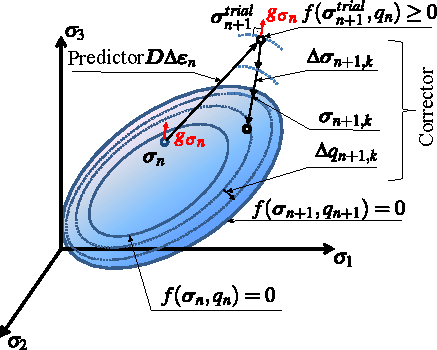
\includegraphics[scale=1]{ep-algorithm-representation.pdf}
	\caption{Illustration of the mapped return semi-implicit with $k$ Newton-Raphson local iterations}
	\label{ep-algorithm-representation}
\end{figure}

Therefore, to solve by Newton-Raphson the system that gives the beginning to the plastic corrector writes in the in the following residual (omitting the index $n+1$):

\begin{equation}
	\label{eq:algoritmo_ep_1}
	\left\{
	\begin{array}{lcl}
		\al = -\strainp + \strainp_n + \Delta \lambda \dgds_n = \zerol	\\
		\bl = -q + q_n + \Delta\lambda\hl_n = \zerol \\
		f = f(\stress,q) = 0
	\end{array}
	\right..
\end{equation}

Linearizing the Eq.~(\ref{eq:algoritmo_ep_1}) in relation to $\Delta \lambda$, knowing that $\Delta \strainp = - \Dsdee^{-1}\Delta\stress$ give:

\begin{equation}
	\label{eq:algoritmo_ep_2}
	\left\{
	\begin{array}{lcl}
		\al_k + \Dsdee^{-1}\Delta\stress_k + \delta \lambda_k \dgds_n = \zerol \\
		\bl_k - \Delta q_k + \delta \lambda_k \hl_n = \zerol \\
		f_k + \dfds_k^T\Delta\stress_k + \dfdq_k^T \Delta q_k = 0
	\end{array}
	\right..
\end{equation}

Eq.~(\ref{eq:algoritmo_ep_2}) comprise a system of three equations with three unkowns: $\Delta \stress_k$, $\Delta q_k$ and $\delta \lambda_k$ and as the flow vectors $\dgds$ and $\hl$ are calculated in the initial step $n$, their gradients did not appear in the formulations. Reorganizing this system we obtain the following solution for the plastic corrector:

\begin{equation}
	\label{eq:algoritmo_ep_3}
	\left\{
	\begin{array}{lcl}
		\Delta \stress_k \\
		\Delta q_k
	\end{array}
	\right\} = -\delta\lambda_k \left[ \All \right]
	\left\{	
	\begin{array}{lcl}
		\dgds_n \\
		\hl_n
	\end{array}
	\right\}
\end{equation}
\begin{equation}
	\label{eq:Ak}
	\left[ \All \right] =
	\begin{bmatrix}
		\Dsdee & \zerol \\
		\zerol & -\onell
	\end{bmatrix}.
\end{equation}
\begin{equation}
	\label{eq:deltalambdak}
	\delta \lambda_k = \dfrac{f_k}{\left[\dfds_k^T~~~~\dfdq_k^T\right]\left[\All \right]\left\{ 
		\begin{array}{lcl}
			\dgds_n \\ 
			\hl_n
		\end{array}\right\}}
\end{equation}

Due to this explicit treatment of the flow vectors in Eq.~(\ref{eq:Ak}), $\left[\All \right]$ presents a closed expression involving only the elastic modulus. In addition, as the system Eq.~(\ref{eq:algoritmo_ep_2}) is composed of linear functions in relation to $\Delta \lambda$ the residuals  $\al_k$ and $\bl_k$ will automatically be null, dispensing its verification in the convergence criterion, as pointed by \citeN{belytschko2000}. 

After updating the stresses and internal variables, it is possible to update the constitutive module. It is possible to use the tangent modulus consistent with the linearization made during the algorithm for integrating the constitutive laws (that is why this modulus is also known as the algorithmic modulus). Its use increase the convergence rate of equilibrium iterations. Its general expression is defined by:
\begin{equation}
	\label{eq:D_alg1}
	\Dsdee^{alg} = \left(\dfrac{d\stress}{d\strain} \right)_{n+1}.
\end{equation}

To derive the expression from $\Dsdee^{alg}$ resolves Eq.~(\ref{eq:esquema_int_constitutiva_ep}) to $d\stress/d\strain$ \cite{belytschko2000}. With that, we have, for elastoplasticity, the following relationship (omitting the $n+1$ index): 
\begin{equation}
	\label{eq:D_alg_ep}
	\Dsdee^{alg} = \Dsdee - \dfrac{\Dsdee~\dgds_n~\dfds^T \Dsdee}{\dfds^T\Dsdee~\dgds_i-\dfdq \hl_n}
\end{equation}
The flowchart can be seen in Fig.~\ref{integração EP semi-implicito}.
\begin{figure}
	\centering
	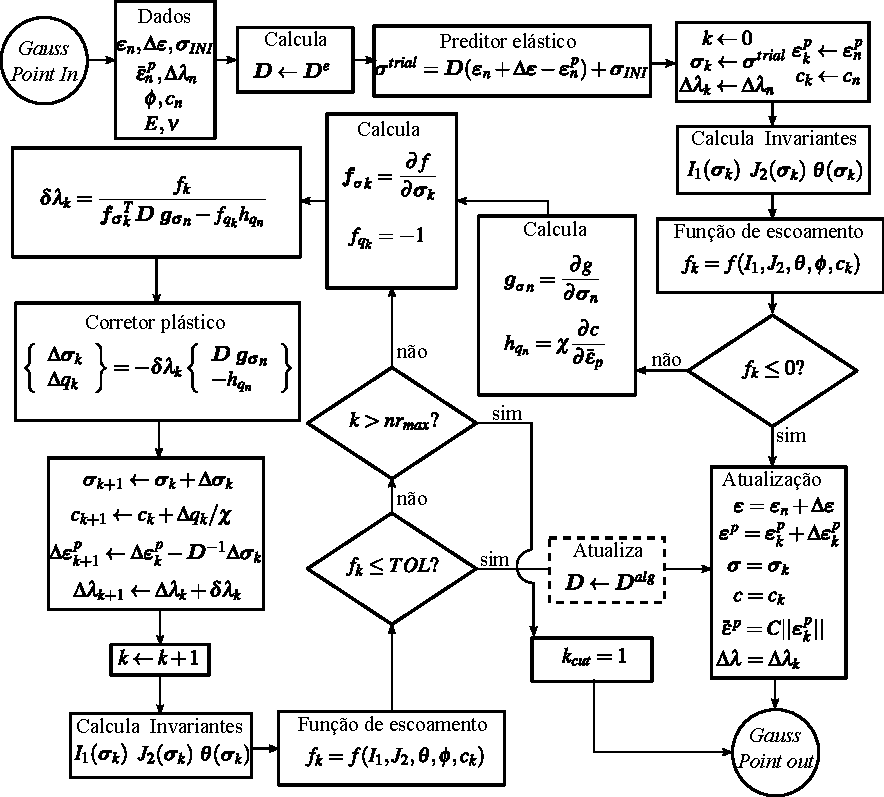
\includegraphics[scale=1]{integração EP semi-implicito.pdf}
	\caption{Integration algorithm for elastoplasticity using a semi-implicit Euler scheme (omitting the index $n+1$)}
	\label{integração EP semi-implicito}
\end{figure}

\subsection{Integration of viscoplastic constitutive equations}

Different integration algorithms can be found in the literature, such as in \citeN{cormeau1975}, \citeN{hughes1978}, \citeN{marques1983}, \citeN{pierce1984}, \citeN{bernaud1991} and some of the most used in \citeN{belytschko2000}, \citeN{souzaneto2008}, \citeN{huang2009} and \citeN{smith2014}. For the present work, a scheme introduced by \citeN{pierce1984}, known as the Rate Tangent Modulus Method, which comprises an explicit Euler scheme for all variables, except for $\Delta \lambda^{vp}$ that is integrated according to the generalized trapezoidal rule. So, we have the following scheme:

\begin{equation}
	\label{eq:esquema_int_constitutiva_vp}
	\left\{
	\begin{array}{lcl}
		\strain_{n+1} = \strain_n + \Delta \strain \\
		\strain_{n+1}^{vp} = \strain_n^{vp} + \Delta \lambda^{vp} \dgds_n^{vp} \\
		q_{n+1}^{vp} = q_n^{vp} + \Delta \lambda^{vp} \hl_n^{vp} \\	
		\stress_{n+1} = \Dsdee~\strain_{n+1}^e = \Dsdee(\strain_{n+1} - \strain_{n+1}^{vp}) \\
		\Delta \lambda = \dfrac{\Delta t}{\eta}[(1-\Theta)\Phi_n + \Theta \Phi_{n+1}]
	\end{array}
	\right..
\end{equation}
Linearizing the overstress of Eq.~(\ref{eq_perzyna_model}) we have:
\begin{equation}
	\label{eq:esquema_int_constitutiva_vp1}
	\Phi_{n+1} = \Phi_n + \dPhidsl_n^T \Delta \stress + \dPhidql_n^T \Delta q^{vp}
\end{equation}
where $\dPhidsl = \partial \Phi / \partial \stress$ e $\dPhidql = \partial \Phi / \partial q$. Replacing  Eq.~(\ref{eq:esquema_int_constitutiva_vp1}) in the Eq.~(\ref{eq:esquema_int_constitutiva_vp})$_5$ we obtain:

\begin{equation}
	\label{eq:esquema_int_constitutiva_vp2}
	\Delta \lambda = \dfrac{\Delta t}{\eta} \Phi_n + \dfrac{\theta \Delta t}{\eta}(\dPhidsl_n^T \Delta \stress + \dPhidql_n^T \Delta q).
\end{equation}
And introducing Eq.~(\ref{eq:esquema_int_constitutiva_vp})$_2$  into Eq.~(\ref{eq:esquema_int_constitutiva_vp})$_4$ and rewriting 
Eq.~(\ref{eq:esquema_int_constitutiva_vp})$_3$ we obtain:
\begin{equation}
	\label{eq:esquema_int_constitutiva_vp3}
	\left\{ \begin{array}{lcl} \Delta \stress \\ \Delta q^{vp} \end{array} \right\} = \left\{ \begin{array}{ccc} \Dsdee(\Delta\strain -\Delta \lambda^{vp} \dgds_n) \\ \Delta \lambda^{vp} \hl_n^{vp} \end{array} \right\}.
\end{equation}
Finally, replacing (\ref{eq:esquema_int_constitutiva_vp3}) in (\ref{eq:esquema_int_constitutiva_vp2}) we can isolate $\Delta \lambda^{vp}$:
\begin{equation}
	\label{eq:esquema_int_constitutiva_vp4}
	\Delta \lambda^{vp} = \dfrac{\Phi_n + \Theta \dPhidsl_n^T\Dsdee\Delta\strain}{\dfrac{\eta}{\Delta t} + \Theta (\dPhidsl_n^T\Dsdee~\dgds_n^{vp} - \dPhidql_n^T \hl_n^{vp})}.
\end{equation}

When $0 < \Theta < 1$ we have a semi-implicit algorithm and when $\Theta = 0$ we have a totally explicit algorithm, with $\Delta \lambda^{vp} = \Delta t \dfrac{\Phi_n}{\ eta}$. As can be seen from this deduction, unlike the integration of the constitutive relationship in elastoplasticity, there is no need to solve the system iteratively. And, in addition, all variables are taken from the previous $n$ substep. This fact, as will be seen in the next section, will facilitate the coupling between the viscoplasticity and elastoplasticity algorithm. Furthermore, for viscoplasticity, hardening-softening laws are not used, simplifying the expression (\ref{eq:esquema_int_constitutiva_vp3}) to:

\begin{equation}
	\label{eq:esquema_int_constitutiva_vp5}
	\Delta \lambda^{vp} = \dfrac{\Phi_n + \Theta \dPhidsl_n^T\Dsdee\Delta\strain_n}{\dfrac{\eta}{\Delta t} + \Theta \dPhidsl_n^T\Dsdee\dgds_n}.
\end{equation}

Substituting (\ref{eq:esquema_int_constitutiva_vp5}) into (\ref{eq:esquema_int_constitutiva_vp3})$_1$ schema gives a closed expression for the stress update:
\begin{equation}
	\label{eq:esquema_int_constitutiva_vp6}
	\Delta \stress = \Dsdee^{alg} \Delta \strain - \boldsymbol p
\end{equation}
with
\begin{equation}
	\label{eq:esquema_int_constitutiva_vp6}
	\Dsdee^{alg} = \Dsdee - \dfrac{\Theta \Dsdee~\dgds_n~\dPhidsl_n^T \Dsdee}{\eta/\Delta t+ \Theta \dPhidsl_n^T\Dsdee~\dgds_n},~~~\boldsymbol p = \dfrac{\Phi_n \Dsdee ~\dgds_n}{\eta/\Delta t+ \Theta \dPhidsl_n^T\Dsdee~\dgds_n}
\end{equation}
where $\Dsdee^{alg}$ is the algorithmic constitutive modulus and $\boldsymbol p$ a pseudo-stress that does not depend on the increment of total strain.

The integration scheme represented by (\ref{eq:esquema_int_constitutiva_vp})$_5$ is unconditionally stable for a value of $\Theta \geq 1/2$. However, this does not guarantee the accuracy of the solution. Thus, as for values $\Theta < 1/2$, a limit value must be used for the time increment $\Delta t \leq \Delta t_{\text{lim}}$. This limit can generally be achieved by reducing the time increment until the solution does not change. Strictly it depends on the material parameters, the integration scheme, the flow surface and the flow rule and there are some analytical solutions for classical surfaces. To avoid this precision problem, in this work, the limits of Drucker-Prager surface is \cite{cormeau1975}:
\begin{equation}
	\label{eq:deltatmin_dp}
	\Delta t_{\text{lim}} \leq \left\{ 
	\begin{array}{lcl} 
		\dfrac{4}{3}\dfrac{\eta}{\Phi}\dfrac{(1+\nu)}{E} {\sqrt{3J_2}} \\
		\dfrac{\eta f_0}{\Phi'}\dfrac{(1+\nu)(1-2\nu)}{E}\dfrac{(3-\sin{\phi})^2}{\frac{3}{4}(1-2\nu)(3-\sin{\phi})^2 + 6(1+\nu)\sin{\phi}^2}
	\end{array} \right.
\end{equation}
where $\phi'= \dfrac{d \phi}{d(f/f0)} = n(f/f0)^{n-1}$. When $\phi = 0$ we have the specific case for the von-Mises surface. This limit is deduced considering the associated viscoplasticity and a fully explicit integration scheme. The flowchart for the viscoplastic equations integration algorithm can be seen in Fig.~\ref{integração VP semi-implicito}.
\begin{figure}
	\centering
		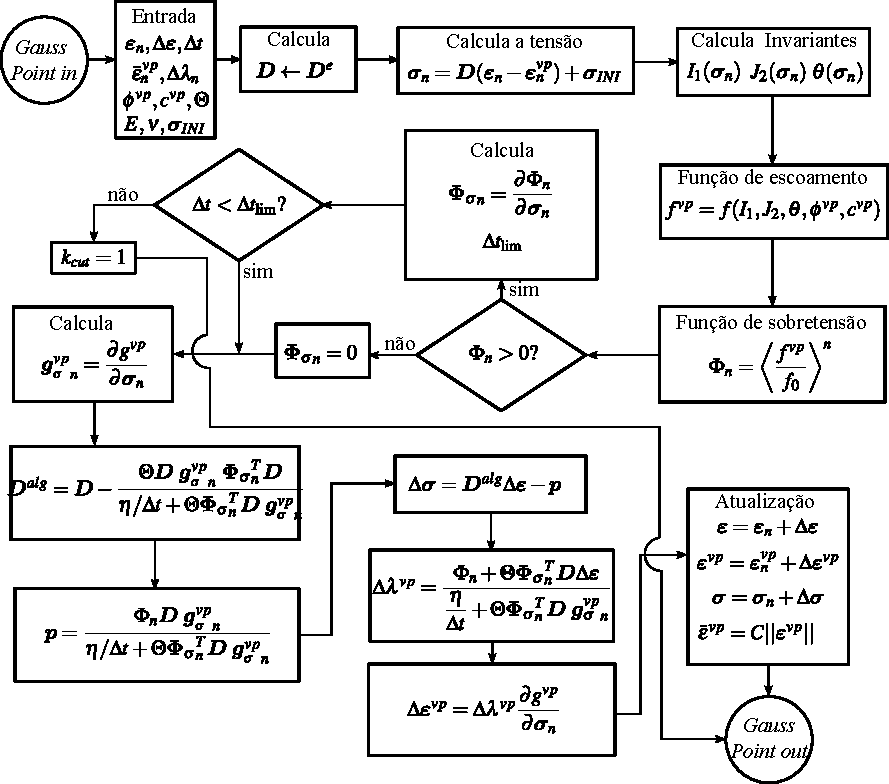
\includegraphics[scale = 1.0]{integração VP semi-implicito.pdf}
	\caption{\label{integração VP semi-implicito}Integration algorithm for viscoplasticity using a semi-implicit Euler scheme without hardening-softening (omitting the index $n+1$).}
\end{figure}

\subsection{Integration of elastoplastic-viscoplastic constitutive equations}

As viscoplasticity is integrated through a semi-implicit rule in which all variables are calculated in substep $n$, that is, with the known stress, the viscoplastic strain increment can be directly discounted from the total strain increment in the elastic prediction step of the elastoplasticity algorithm. The algorithm for integrating the elastoplastic-viscoplastic constitutive equations can be seen in the flowchart of Fig.~\ref{integração EPVP}.

\begin{figure}
	\centering
	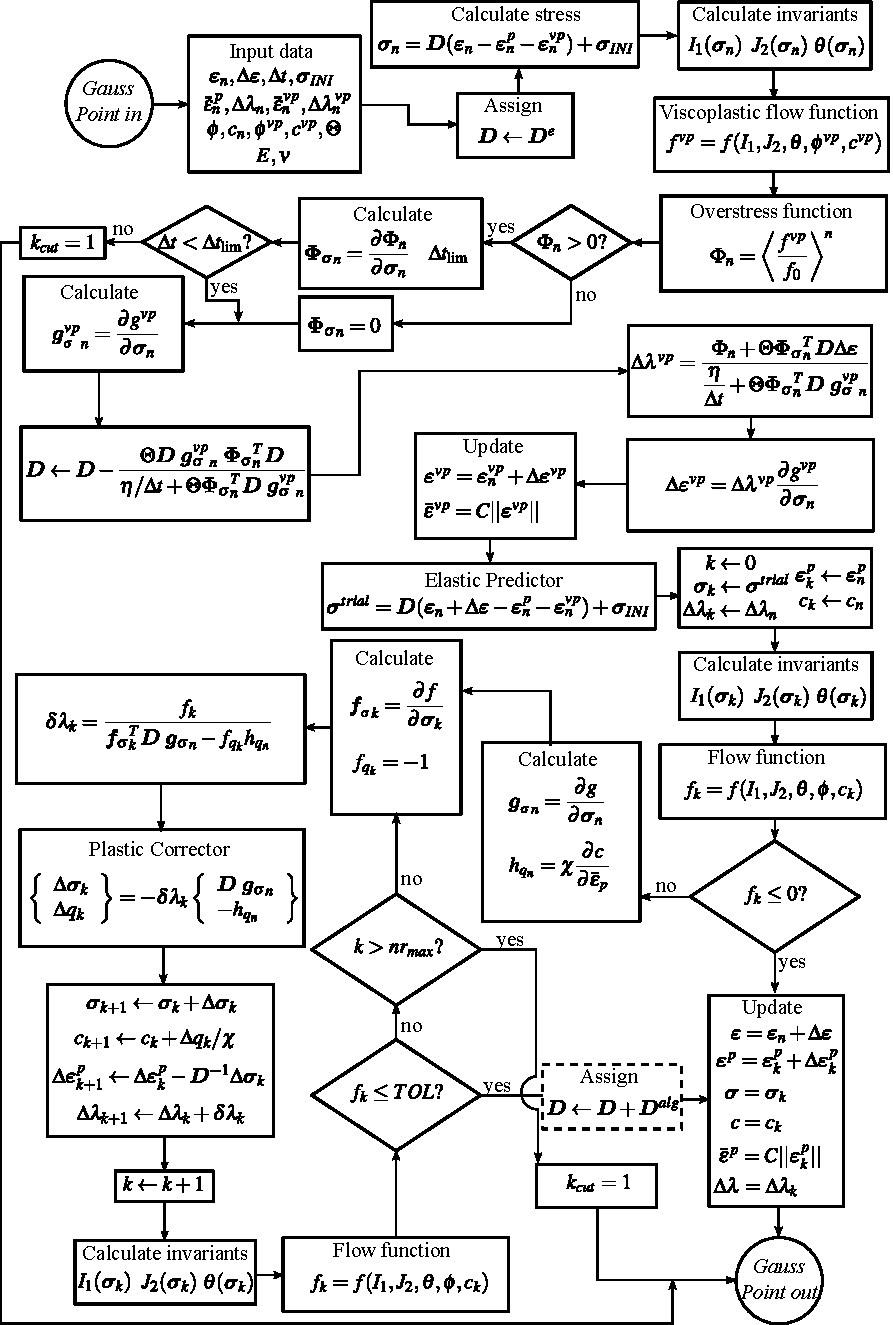
\includegraphics[scale = 1.0]{integração EPVP.pdf}
	\caption{\label{integração EPVP}Integration algorithm for elastoplasticity-viscoplasticity (omitting the index $n+1$).}
\end{figure}

\section{Validation of the model}

As validation, a comparison will be made with the analytical and numerical solution deduced by \cite{piepi1995} for a perfect elastoplastic-viscoplastic model with Tresca’s criterion applied to deep clay rockmass. This analytical solution was chosen because it uses the same association principle as in Fig.~\ref{reological_scheme} and will be compared with the numerical solution in axisymmetry. Furthermore, it is considered the same surface for plasticity and viscoplasticity, and their flow vectors are fully associated  $f^p = g^{p} = f^{vp} = g^{vp}$. 

The algorithm was implemented in ANSYS software through the UPF (User Programming Features). The mesh (Fig.~\ref{malhaAXI}) comprises 1222 linear elements of four nodes, two degrees of freedom per node and four integration points. The domain was divided into four areas to control spatial discretization. The system size, after applying the boundary conditions is of 7626 equations. The excavation method consisted of the technique of deactivating the elements to be excavated by multiplying the modulus of elasticity by $10^{-16}$ (eliminating its contribution to the stiffness matrix) and making the stresses to zero in the Gauss points during the integration of internal forces. The geometric parameters are in Tab.~\ref{parametros_AXI}.

\begin{figure}
	\centering
	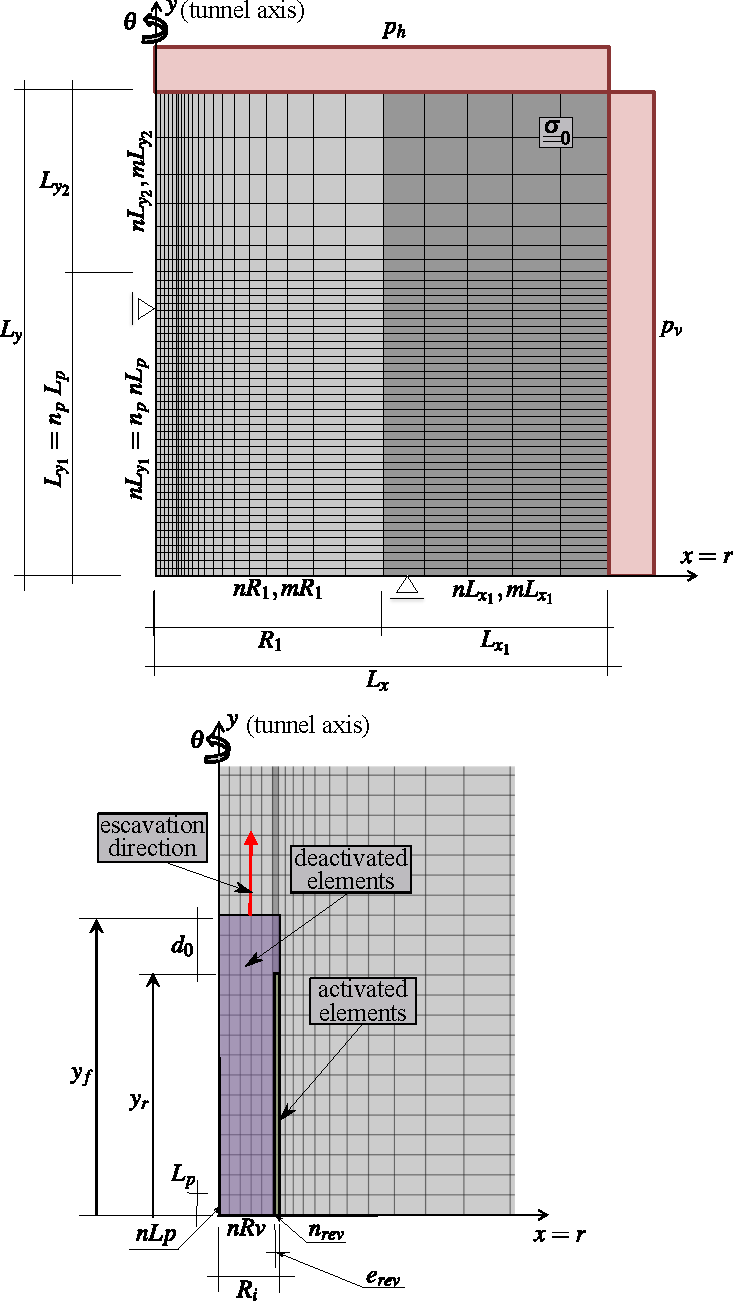
\includegraphics[scale = 1.0]{malhaAXI.pdf}
	\caption{\label{malhaAXI}Domain, parameters, boundary conditions and the mesh of the axisymmetric numerical model.}
\end{figure}

\begin{table}
	\caption{Geometric parameters of the mesh}
	\label{parametros_AXI}
	\centering
	\small
	\renewcommand{\arraystretch}{1.25}
	\begin{tabular}{c c c c}
		\hline
		\multicolumn{1}{c}{\textbf{PARAMETERS}} &
		\multicolumn{1}{c}{\textbf{SYMBOL}} &
		\multicolumn{1}{c}{\textbf{UNIT}} &
		\multicolumn{1}{c}{\textbf{VALUES}} \\
		\hline
		\multicolumn{4}{c}{GEOMETRIC DOMAIN} \\
		\hline
		Radius of interface between tunnel and rockmass & $R_i$ & m & 1 \\		
		Lining thickness & $e_{rev}$ & m & 0,1 \\
		Radius of the region near the tunnel $R_1$ & $R_1$ & m & 10$R_{i}$ \\
		Total domain lenght & $L_{x}$ & m & $20R_i$ \\		
		Length beyond $R_1$ & $L_{x_1}$ & m & $L_x - R_1$ \\							
		\hline
		\multicolumn{4}{c}{ESCAVATION AND PLACEMENT OF LINING} \\
		\hline
		Number of excavation steps & $n_p$ & un & 38 \\
		Numeber of steps in first excavation & $n_{p_i}$ & un & 3 \\
		Length of the excavated part & $Ly_{1}$ & m & $n_pL_p$ \\
		Length of unexcavated part & $Ly_{2}$ & m & $25L_p$ \\
		Longitudinal length of domain & $L_y$ & m & $L_{y_1}+L_{y_2}$ \\
		Excavation step size & $L_{p}$ & m & $1/3R_{i}$ \\
		Unsupported dimension & $d_0$ & m & $0,~2L_{p},~4L_{p}$ \\
		Lining face coordinate & $y_r$ & m & $(i_p-1)L_p + n_{p_i}L_p - (L_p+d_0)$ \\
		Excavation face coordinate & $y_f$ & m & $(i_p-1)L_p + n_{p_i}L_p$ \\
		\hline
		\multicolumn{4}{c}{DISCRETIZATION} \\
		\hline
		Elements along $R_i$ & $nR_{i}$ & un & 5 \\	
		Elements in lining thickness & $n_{rev}$ & un & 2 \\			
		Elements along $R_1$ & $nR_{1}$ & un & 15 \\	
		First and last element ration of $R_1$ & $mR_{1}$ & adm & 15 \\	
		Elements along $L_{x_1}$ & $nL_{x_1}$ & un & 5 \\
		First and last element ration of $L_{x_1}$ & $mL_{x_1}$ & adm & 5 \\				
		Element size in excavated part & $L_{p_e}$ & m & $L_{p}$ \\	
		NNumber of elements along $L_{y_2}$ & $nL_{y_2}$ & un & 8 \\			
		First and last element ratio of $L_{y_2}$ & $mL_{y_2}$ & adm & 5 \\				
		\hline
	\end{tabular}
	\normalsize
\end{table}

The following constitutive parameters are used: $E=1500$MPa and $2000$MPa, $\nu=0.498$, $c^i=c^p=c^r =4\sqrt{3}/2$MPa, $ c^{vp}=3\sqrt{3}/2$MPa, $\eta = 4 \cdot 10^4$day, $n=1$, $f_0=1$MPa and $p_v=p_h=9$ MPa. The viscous phenomenon evolves over time between excavation steps. This time is calculated as the ration between the step size of the excavation $L_p$ and the excavation speed $V_p = 10m/day$. After the last excavation the model continues incrementing the time until the deformation increment is in the order of $10^{-8}$. In the latter, it can be noted that the elastoplastic model has greater cohesion than the viscoplastic model. This causes viscoplastic deformations to start even before the solid plasticize. The long-term convergence profile, that is, after the time-deferred effects cease, can be seen in Fig.~\ref{convergence_profile_piepi} and Fig.~\ref{convergence_profile_piepi_with_lining}. There is an excellent agreement between the proposed numerical solution with the analytical and numerical solution given by \citeN{piepi1995}.

\begin{figure}
	\centering
	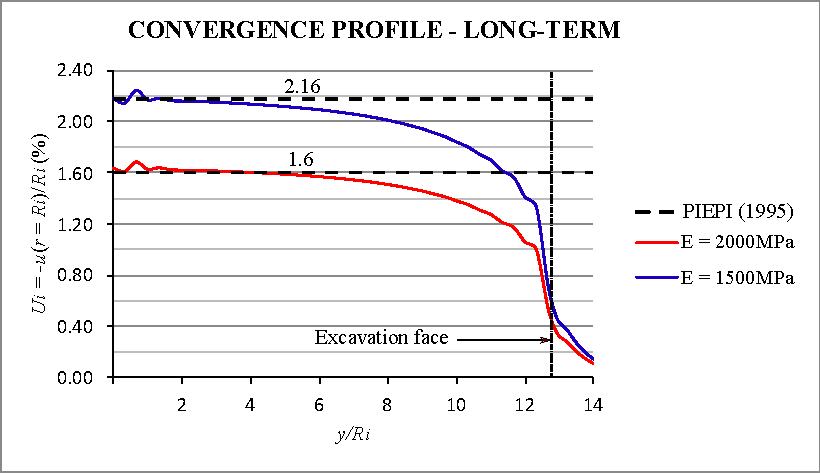
\includegraphics[scale = 1.0]{convergence_profile_piepi.pdf}
	\caption{\label{convergence_profile_piepi}Verification with Piepi (1995) analytical solution of the model elastoplastic-viscoplastic without lining.}
\end{figure}

\begin{figure}
	\centering
	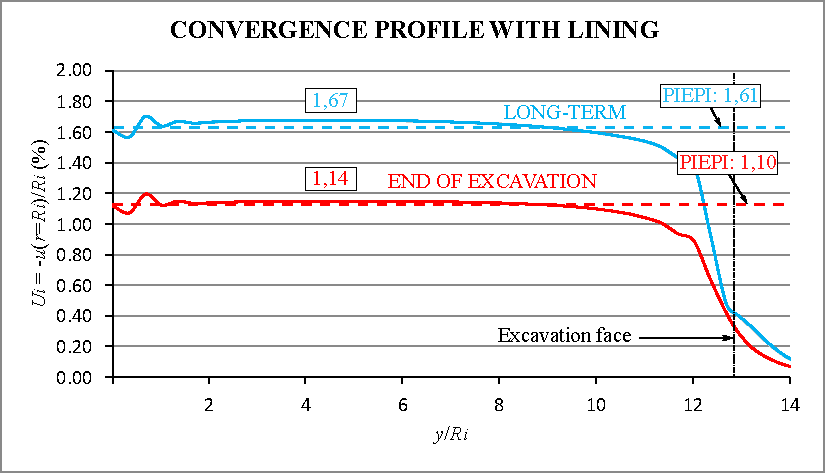
\includegraphics[scale = 1.0]{convergence_profile_piepi_with_lining.pdf}
	\caption{\label{convergence_profile_piepi_with_lining}Verification with Piepi (1995) numerical solution of the model elastoplastic-viscoplastic with lining.}
\end{figure}

\begin{figure}
	\centering
	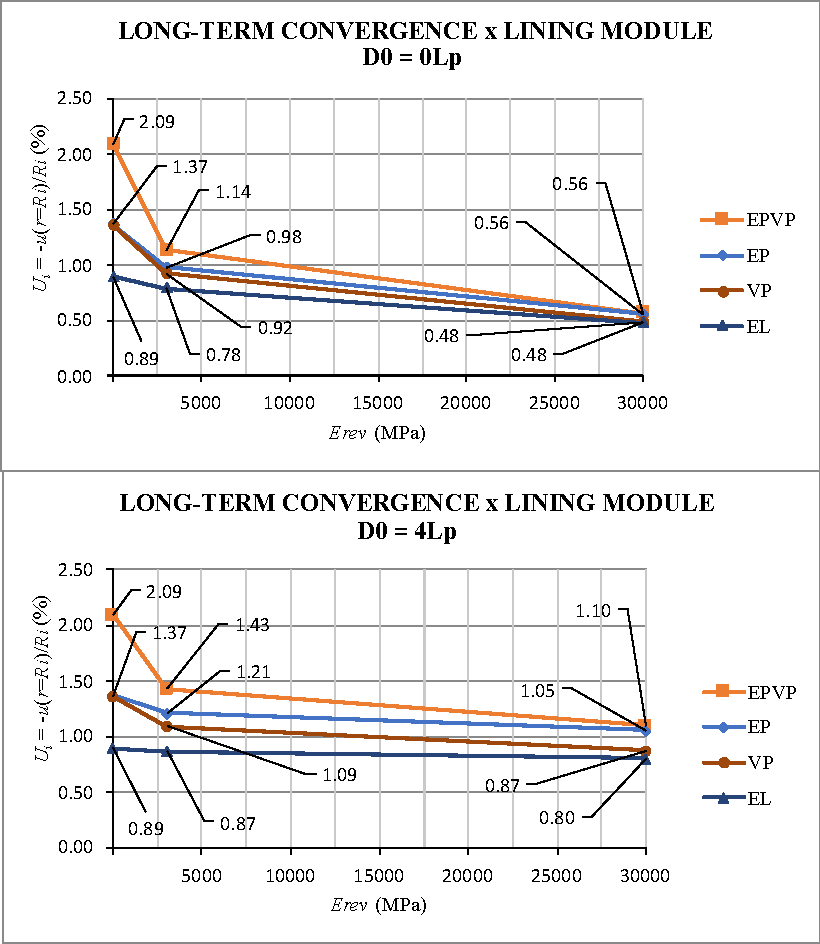
\includegraphics[scale = 1.0]{convergence_lining_module.pdf}
	\caption{\label{convergence_lining_module}Long-term convergence versus lining modulus of elasticity for an unsuported distance $d0=0$ and $d0=4L_p$.}
\end{figure}


%De modo a verificar o algoritmo acoplado implementado é feita a comparação com a solução analítica deduzida por \citeonline[p. 61]{Piepi1995} para um túnel profundo em condições geostáticas-hidrostáticas no interior de um maciço com comportamento elastoplástico-viscoplástico perfeito obedecendo ao critério de Tresca. Essa solução analítica foi escolhida por utilizar o mesmo princípio de associação da \autoref{lei_endurecimento_rousset}, como pode ser visto em \citeonline[p. 35]{Piepi1995}. Contudo, não apresenta a mesma generalidade da solução numérica implementada e possui algumas hipóteses simplificativas, dentre elas, a consideração da mesma superfície de escoamento para plasticidade e viscoplasticidade e vetores de fluxo totalmente associados, ou seja, $\fl^p = \gl^{p} = \fl^{vp} = \gl^{vp}$. Para essa verificação é utilizado o modelo axissimétrico com os seguintes parâmetros: $E=1500$MPa e $2000$MPa, $\nu=0,498$, $c^i=c^p=c^r =4\sqrt{3}/2$MPa, $c^{vp}=3\sqrt{3}/2$MPa, $\eta = 4 \cdot 10^4$dia, $n=1$, $f_0=1$MPa e $p_v=p_h=9$MPa. Esses parâmetros são os mesmos utilizado por \citeonline[p. 131]{Piepi1995} que chegou nas convergências de $U_i=2,16$\% para $E=1500$MPa e $U_i=1,6$\% para $E=2000$MPa.

\section{Parameters for analyzes}

\section{Results and Discussion}



\section{Conclusions}


\section{Data Availability Statement}

Some or all data, models, or code that support the findings of this study are available from the corresponding author upon reasonable request. (ANSYS APDL script for FEM model and USERMAT suboroutine in FORTRAN90 for constitutive concrete model)

\pagebreak
%
% Now we start the Appendixes, with the new section name, "Appendix", and a 
%  new counter, "I", "II", etc.
%\appendix
%
%
% Now we start the appendices, with the new section name, "Appendix", and a 
%  new counter, "I", "II", etc.
%\appendix
%
% And now for some pretty impressive notation.  In this example, I have used
%   the tabular environment to line up the columns in ASCE style.
%   Note that this and all appendices (except the references) start with 
%   the \section command
%
%
% Here's the list of references:
%
% \label{section:references}
\bibliography{ascexmpl-new}
%

\end{document}
